%Architecture montrant le découpage des différents modules logiciels et matériels et leurs interactions dynamiques (diagramme UML : composants, déploiement, séquence)
%Spécification d'interface entre les composants
%Sécurité


\subsection{Architecture Globale}
De façon globale, on peut voir le système final comme l'assemblage de 3 grands modules, eux mêmes composés de sous modules. 
Nous avons donc:
\begin{itemize}
	\item Extraction du texte brut
	\item Extraction de métadonnées et ajout de taxonomies
	\item Indexage et Moteur de recherche
\end{itemize}

\subsubsection{Interfacage}

\subsection{Extraction du texte brut}
La majorités des documents que nous avons pu obtenir était sous format .pdf.
Ce format est hautement portable, et est très couramment utilisé.
Pour pouvoir analyser correctement ces documents, nous devions extraire le texte inclus dans ces fichiers.
Ce texte sera ensuite utilisé pour l'extraction des métadonnées et l'ajout de taxonomie. Selon la façon dont le fichier a été enregistré, et les objets contenus (tableaux, images), la qualité de l'extraction du texte peut fortement varié. 

Nous utilisons une approche double, qui nous assure une haute qualité d'extraction avec un temps d'exécution raisonnable.
A l'aide d'un script bash, nous listons tout les fichiers disponibles dans le dossier initial donné par l'utilisateur. 

Nous utilisons d'abord un utilitaire appelé "pdftotext" qui tente d'abord une extraction simple en analysant le fichier pdf.
Il se peut cependant que cette approche faille a extraire le texte demandé.
Dans ce cas, nous avons développé une approche basé sur Tesseract, un programme d'OCR (Optical Character Recognition) développé en partie par Google. 

L'OCR tente d'extraire du texte depuis une image.
Les techniques actuelles se basent sur des modèles de Deep Learning tels que le LSTM et les CNNs, qui vont essayer de localiser les zones de textes et d'en tirer les caractères présent.
Cette approche, bien que souvent efficace, peut également faillir, et donner en sortie des caractères éronnés.
La qualité du texte extrait étant critique pour le reste du projet, beaucoup de soins ont été donnée dans le pré traitement du fichier pdf pour obtenir une qualité d'extraction optimale.

\begin{figure}[h!]
  \centering
	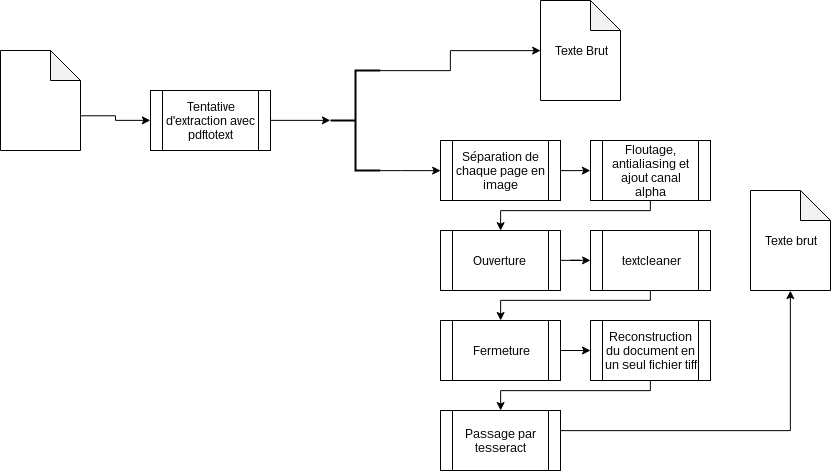
\includegraphics[width=0.7\textwidth]{extractionText.png}
	\caption[]{Diagramme fonctionnel du module d'extraction du texte}
  \label{}
\end{figure}


\subsection{Module taxonomique}

\begin{figure}[h!]
  \centering
  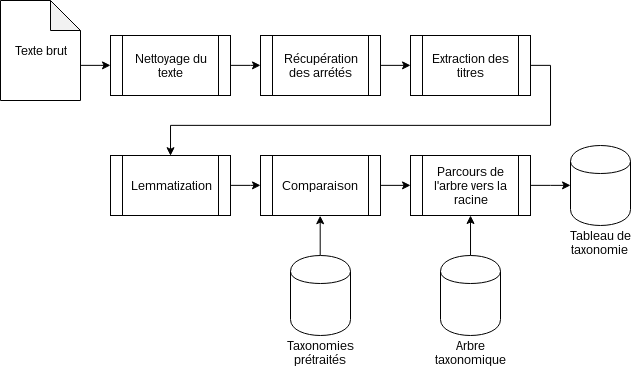
\includegraphics[width=0.8\textwidth]{diagArchiTaxo.png}
	\caption[]{Diagramme de l'architecture du module taxonomique}
  \label{}
\end{figure}


Le module taxonomique a pour charge d'extraire et d'assigner une ou plusieurs taxonomie a un document.
Pour des raisons d'efficacité et de précision, ce module extrait d'abord le titre des arrêtés administratifs contenu dans le texte, puis les compare avec les taxonomies après une normalisation.
Cette normalisation consiste en un nettoyage des accents et caractères spéciaux, ainsi qu'une lemmatization, procédure où l'on remplace un mot par sa racine.
Ces opérations permettent une comparaison plus robuste et moins dépendante du contexte de la phrase. 

Pour chaque mot de la taxonomie, le module va vérifier si celui ci est présent dans le titre qu'il est en train d'analyser.
Si oui, ce mot est ajouté a la taxonomie du document.

Pour obtenir une taxonomie plus vaste, nous prenons également en compte la structure de la taxonomie.
En effet, celle ci se présente sous forme d'un arbre, structure que nous pouvons observer en figure \ref{fig:tree}.
Chaque sections possèdes des sous sections, qui permettent un affinage et une grande précision dans la classification.
L'idée principale étant de considérer que si un document possède comme taxonomie une feuille ou un noeud de cette arbre, alors il doit nécessairement posséder comme taxonomie tout les parents de ce noeud.
Nous remontons donc jusqu'à la racine de l'arbre depuis le noeud, en ajoutant a la taxonomie du document tous les noeuds que nous rencontrons en chemin.
Cette approche nous permet d'obtenir une plus grande variété de taxonomie sans avoir a utiliser une analyse plus lourde sur le texte.
De plus ces taxonomies, parce qu'elles sont des parents de la taxonomie initiale, sont des sur-ensembles.
\begin{figure}[h!]
  \centering
  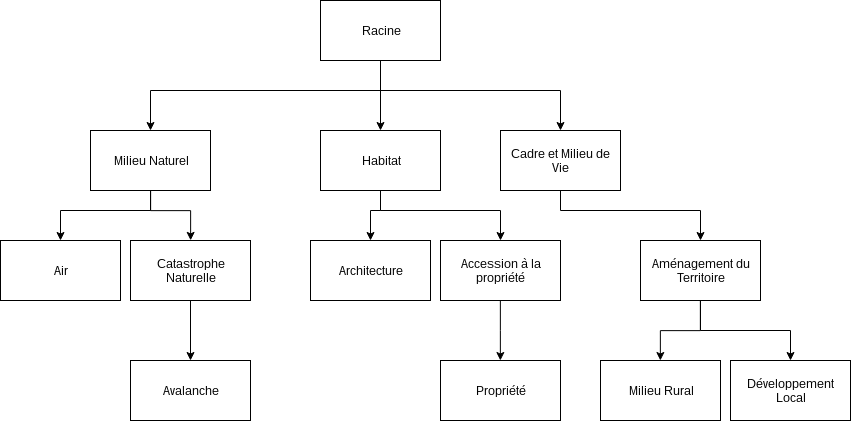
\includegraphics[width=0.8\textwidth]{TaxoTree.png}
	\caption[]{Aperçu de l'arbre taxonomique}
  \label{fig:tree}
\end{figure}

\subsection{Extraction des métadonnées}
Les métadonnées sont des informations \textit{concernant} le document.
Nous avons choisi de construire des modules spécialisés, chacun ayant pour rôle d'extraire un type de métadonnées particulère.
Cette spécialisation nous permet de facilement ajouter des types de métadonnées a la sortie finale et respecte une volonté de compartementalisation des responsabilités du programme: pour chaque type d'information a extraire du texte, i.e\. taxonomie, numéro d'article, date de publication, un module lui est dédié. 

Pour le cas de la taxonomie, le schéma global de fonctionnement est le suivant: une fonction d'ajout de métadonnées au fichier .json appelle chaque fonction d'extraction individuellement.
La figure \ref{globalMeta} représente un diagramme fonctionnel général de l'extraction de métadonnées. 
Ces fonctions sont généralement courtes et consiste de regex spécialement construite pour extraire l'information demandé.
Pour rappel, une regex est une séquence de caractère définissant un critère de recherche précis.
Ces fonctions ont l'avantage d'être extrêmement rapide, avec un temps d'execution dans les millisecondes, mêmes pour des documents ayant des centaines de pages. 

\begin{figure}[h!]
  \centering
	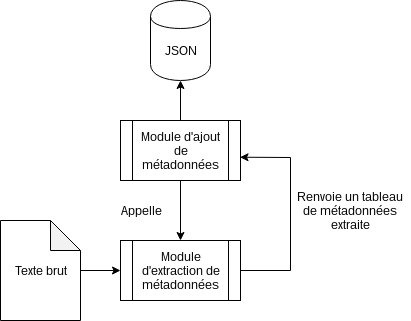
\includegraphics[width=0.5\textwidth]{SchemaGlobal.png}
	\caption[]{Diagramme fonctionnel général des fonctions permettant l'extraction des métadonnées}
  \label{fig:globalMeta}
\end{figure}

Chacune de ces fonctions prends en entrée le texte brut initial, et ressort un tableau de métadonnées extraite.
Ces tableaux sont ensuite directement insérées dans le fichier JSON, qui constitue la base sur lequel le moteur de recherche fonctionne.



\subsection{Moteur de recherche avec Reactivsearch/Appbase.io}
Appbase est le site qui va centraliser l'ensemble des données et les rendre visible à travers une première version d'interface.
Le module moteur de recherche fonctionne indépendamment des autres modules. Une fois les métadonnées et la taxonomie importés dans le format Json, le elasticsearch effectue l'indexation. Avec reactivsearch il existe plusieurs modules tels que les champs de recherche avec l'autosuggestion ou l'ajout des filtres.  

Afin d'importer nos données, nous devons respecter le format JSON.
Dans un premier temps, nous créons une application depuis Appbase.io. 
Un Json se compose de plusieurs documents où chaque document est enlacé par des accolades. Dans un document, nous avons des "fields" (champs) qui correspondent aux différentes familles de données récoltés. Dans notre cas, nous avons comme exemple de champs les noms, les arrêtés ou les numéros de recueils. La structure du JSON est la suivante :


\begin{figure}[h!]
  \centering
	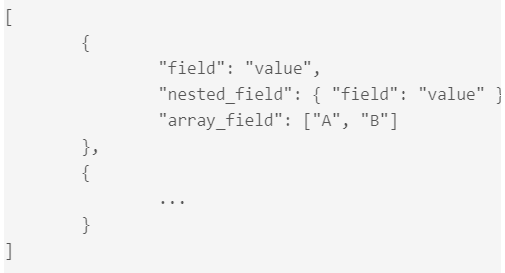
\includegraphics[width=0.5\textwidth]{FormatJsonAppbase.PNG}
	\caption[]{Exemple format JSON}
  \label{}
\end{figure}

Lorsque les données sont correctement importées un mail est envoyé contenant le "credentials" (identifiant) afin de sécuriser l'accessibilité aux données et visibles sous la forme d'un tableau. Cela nous permet de visualiser ce qui a été importé. 

\begin{figure}[h!]
  \centering
	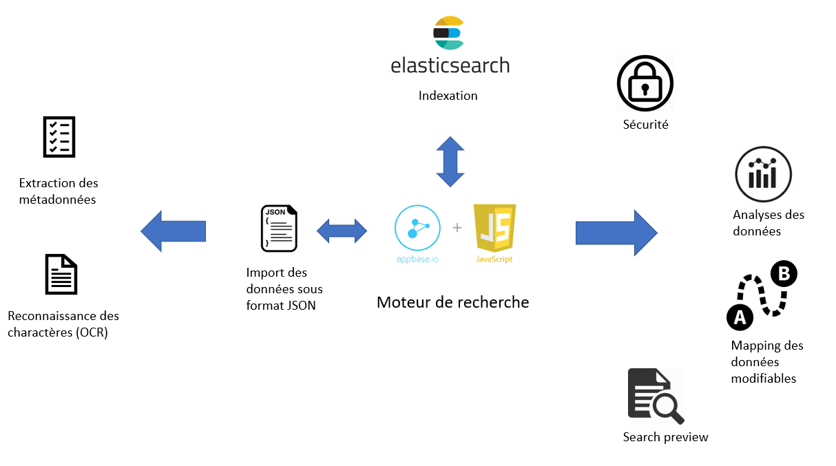
\includegraphics[width=0.5\textwidth]{SpecTechArchiMoteur.png}
	\caption[]{Diagramme fonctionnel du moteur de recherche}
  \label{}
\end{figure}

Depuis l’onglet « search preview » nous avons une première visualisation du moteur de recherche. Avec la bar de recherche généré, nous pouvons spécifier les champs qui sont recherchables. 
Le résultat des recherches se composent d’un titre, d’une description et d’une url que nous ajoutons. De plus, nous avons la possibilité d’ajouter des filtres. Ils permettent de spécifier le type de recherche que nous souhaitons.

Il existe CodesSandbox qui permet d’avoir accès au code javascript généré par appebase.io. Ce dernier a la particularité d’être multiplateforme et de nous donner accès un lien d’acces web vers l’application.


\subsection {Utilisation globale}
%detail de l'utilisation 
%parcours de l'ajout pdf jusqu'au site internet

